\PassOptionsToPackage{xetex,dvipsnames}{xcolor}
\PassOptionsToPackage{xetex}{graphicx}
\documentclass[xetex]{beamer}  % ue6aue6a
\title[Wordnets and Metaphor]{Multilingual Modelling with Wordnets:
  \\ Metonymy Travels, Metaphor Wanders}
%\\[2ex] \bl{Picking Brains, Crossing Ideas}}
\author[Bond and many more]{Francis \textbf{Bond} 
  \\ and many, many more}
\institute[Palacký]{General Linguistics and Asian Studies,
\\  Palacký University, Olomouc, Czechia
\\[1.5ex] \url{<bond@ieee.org>}}

\date[2026]{2026 Schultink Winter Lecture} %%% FIXME
\newcommand{\ili}[1]{\href{http://www.globalwordnet.org/ili/#1}{\url{#1}}}

%%% make it smaller
 % gs -sDEVICE=pdfwrite -dCompatibilityLevel=1.4 -dPDFSETTINGS=/printer -dNOPAUSE -dQUIET -dBATCH -sOutputFile=omw-teanga-small.pdf omw-teanga.pdf 
\usepackage{chainnet}
\usepackage{booktabs}
\newcommand{\clex}[1]{\textbf{\texttt{#1}}}
\newcommand{\ldiff}[1]{\textbf{\texttt{#1}}}
\newcommand{\dom}[1]{\textbf{\texttt{#1}}}

\newcommand{\LEX}[6][]{\textbf{\textit{#2}} \textit{#1} (#3: #4) #5 --- \textit{#6}}

\usepackage{tcolorbox}
% Define your custom style
\tcbset{
    lightbox/.style={
        boxsep=2pt,
        colback=blue!5!white,
        colframe=gray!20,
        boxrule=0.2pt,
        width=0.3\textwidth
    }
}\tcbset{
    fullbox/.style={
        boxsep=2pt,
        colback=blue!5!white,
        colframe=gray!20,
        boxrule=0.2pt,
        width=\textwidth
    }
}
\newcommand{\onew}[1]{\hspace*{-0.5em}\colorbox{black!20}{#1}}

\newcommand{\wns}[2]{\textit{\textbf{#1}}\,\ensuremath{_#2}}

%\usepackage[hidelinks]{hyperref}
\hypersetup{ 
     colorlinks, 
     linkcolor={blue!50!black},
     citecolor={red!50!black},
     urlcolor={blue!80!black}
}


\usepackage{array}
\newcolumntype{H}{>{\setbox0=\hbox\bgroup}c<{\egroup}@{}}

\usepackage[round]{natbib}
\usepackage{fontenc}
\usepackage{polyglossia}
\setmainlanguage{english}
\usepackage{xeCJK}
%\setCJKmainfont{WenQuanYi Micro Hei}
% \setmainfont[Numbers=OldStyle]{TeX Gyre Pagella}
%\setCJKmainfont{Droid Sans Fallback}
\setCJKmainfont{Noto Sans CJK SC}
\usefonttheme{professionalfonts}
\setsansfont{Linux Libertine O}
\logo{NTU}
\logo{
\includegraphics[width=15mm]{img/UP_logo_FF_horizont_en.png}}

 \usepackage{qtree,avm,expex}
\definelingstyle{cmn}{everygla=,
everyglb=\itshape,everyglc=\footnotesize}

\usepackage{relsize,xspace}


\usetheme{Boadilla}
\usecolortheme{seahorse}
\setbeamertemplate{navigation symbols}{}

\newcommand{\zhong}{\ensuremath{[\Big|]}}
% NUS Meeting Room 1 (MR 1) 	COM1-03-19
\newcommand{\bl}[1]{\textcolor{blue}{#1}}
%\newcommand{\sh}[1]{\textcolor{blue}{#1}}
\newcommand{\txx}[1]{\textbf{\textcolor{blue}{#1}}}
\usepackage{url}

%\newcommand{\wn}{\url}
\usepackage[e,f,j]{mtg2e}
\newcommand{\cmn}{\mtciteform}
\newcommand{\kor}{\mtciteform}
\renewcommand{\mtcitestyle}[1]{\textcolor{teal}{\textit{#1}}}
\usepackage{xcolor}
 \newcommand{\bs}{\textbackslash}   % backslash
 \newcommand{\cmd}[1]{{\bf \color{red}#1}}   % highlights command
 \newcommand{\wemp}[1]{\ul{#1}}   % highlight
 \newcommand{\emp}[1]{\textbf{\color{blue}{#1}}}   % highlight
 \newcommand{\rel}[1]{\textsc{\color{blue}{#1}}}
 \newcommand{\lnk}[1]{\rel{#1}}
 \newcommand{\dff}[1]{\texttt{\color{blue}{#1}}}

 \newcommand{\lex}[1]{\textbf{\color{teal}{\textit{#1}}}}
 \newcommand{\lng}[1]{\textcolor{teal}{\textit{#1}}}
\newcommand{\wn}[3]{\lex{#1}\ensuremath{_{#2:#3}}}
\usepackage{relsize}
\newcommand{\wnida}[1]{\asort{\wnid{#1}}}
\newcommand{\wnid}[1]{\textsf{\smaller #1}}

\usepackage{mygb4e,url}
\usepackage[normalem]{ulem}
\newcommand{\ul}{\uline}
\newcommand{\ull}{\uuline}
\newcommand{\udl}{\dashuline}
\newcommand{\uwl}{\uwave}

\newcommand{\MyLogo}[1]{(#1)}

\newcommand{\sh}[1]{https://fcbond.github.io/sh-canon/#1.html}
\newcommand{\SCAN}{\href{\sh{scan}}{\textit{A Scandal in Bohemia}}\xspace}
\newcommand{\REDH}{\href{\sh{redh}}{\textit{The Redheaded League}}\xspace}
\newcommand{\HOUN}{\href{\sh{houn}}{\textit{The Hound of the
      Baskervilles}}\xspace}
\newcommand{\SPEC}{\href{\sh{spec}}{\textit{The Adventure of the Speckled Band}}\xspace}
\newcommand{\DANC}{\href{\sh{danc}}{\textit{The Adventure of the Dancing Men}}\xspace}
\newcommand{\FINA}{\href{\sh{fina}}{\textit{The Adventure of the Final Problem}}\xspace}
\newcommand{\NAVA}{\href{\sh{nava}}{\textit{The Adventure of the Naval Treaty}}\xspace}

\newcommand{\swn}{SentiWordNet\xspace}
\newcommand{\plwn}{plWordNet\xspace}
\newcommand{\plemo}{plWordNet~emo\xspace}
\newcommand{\pwn}{Princeton WordNet\xspace} 
\newcommand{\mlsc}{ML-SentiCon\xspace}
\newcommand{\wnop}{\textsc{Micro-WNOp}\xspace}
\newcommand{\ntumc}{NTU-MC\xspace}


\begin{document}
\maketitle
\lingset{lingstyle=cmn}
\begin{frame}{Outline}
   \tableofcontents
 \end{frame}


\section{Metaphor}
\begin{frame}{Metaphor and Metonymy}

  \begin{itemize}
  \item Metaphor and Metonymy are two fundamental tropes (figures of speech)
  \item Both play crucial roles in the way we understand and use language
  \item \txx{Metaphor} involves understanding one concept in terms of
    another, often unrelated, concept.
     \begin{itemize}
    \item \eng{This horse has a \ul{chestnut} on its leg} ``a small horny bump''
    \item Metaphors create new concepts in the target domain by
      mapping elements from the source domain
    \end{itemize}
    \item They are crucial in understanding novel uses of words
  \item \txx{Metonymy} involves the substitution of one term for
    another to which it is closely related
    \begin{itemize}
    \item \eng{I ate a \ul{chestnut}}
    \item \eng{I pruned the \ul{chestnut} [tree]}
    \item \eng{This table is made from \ul{chestnut} [wood]}
    \item Metonymy works by contiguity or association between concepts,
      usually by some shared attribute, or by a part-whole relation
    \end{itemize}
  \end{itemize}

\end{frame}


\begin{frame}{The state-of-the art}

  \begin{itemize}
  \item Conceptual Metaphor research very wide spread (cognitive, computational, therapeutic, political)
    \begin{itemize}
    \item A lot of fantastic research!
    \end{itemize}
  \item No broad coverage multilingual inventory of metaphors
    \begin{itemize}
    \item MetaNet --- long-running but mainly English (some Spanish and Chinese, far from comprehensive)
    \item \href{https://metaphorshare.com/}{MetaphorShare} --- new
      (2025) initiative to bring together resources, but most with only
      hundreds or thousand of examples.
    \end{itemize}
  \item No broad coverage multilingual corpora of instances
    \begin{itemize}
    \item MIPVU is the largest (mainly English, some work in other languages)
    \end{itemize}
  \item No broad coverage multilingual metaphor interpretation tools
    \begin{itemize}
    \item Some tools for identification
    \item Some tools for paraphrasing, but biased toward English (LLMs)
    \end{itemize}
  \end{itemize}
  
\end{frame}


\begin{frame}{SoA: scattered fragments of the metaphor landscape}
  \centering
  
\includegraphics[width=0.95\textwidth]{img/bond_metaphor_diagram_1.png}
%  \caption{The state-of-the-art: scattered fragments of the metaphor landscape}\label{fig:fragment}
\end{frame}

\begin{frame}{We are trying a different approach}
  \begin{itemize}
  \item Exploit existing multilingual resources (wordnets and sense-annotated corpora)
  \item ChainNet links word senses by metaphor --- for all$^*$ nouns in the English wordnet
  \item Use ChainNet to study metaphor over a (quite) complete vocabulary
    \begin{itemize}
    \item Link lexical to conceptual metaphors
    \item Find unknown conceptual metaphors (unlinked lexical metaphors)!
    \item \textbf{Finish with a much more complete understanding}
    \item Use wordnet sense tagged corpora to investigate attested uses
    \item \textbf{Finish with a grounded, quantitative understanding}
    \end{itemize}
  \end{itemize}
\end{frame}




\section{ChainNet}
\label{sec:chainnet}



\begin{frame}{ChainNet}

  \begin{itemize}
  \item ChainNet is an attempt to comprehensively model these tropes \citep{maudslay-etal-2024-chainnet-structured,Bond:Maudslay:2025}
    \begin{itemize}
    \item All nouns (word + synset combinations) in the
      Princeton Wordnet 3.0 \citep{_Fellbaum:1998} with three or more senses$^*$
      were annotated
    \item Every sense linked to another sense, or treated as a homonym (unrelated)
      \begin{itemize}
      \item 7,500 metaphor pairs
      \item 6,116 metonymy pairs
      \end{itemize}
  \item Most annotated by 1 annotator, some by 2 annotators
    \begin{itemize}
    \item Inter-annotator agreement 70\% (88\% for same prototype)
    \item Intra-annotator agreement 81\% (92\% for same prototype)
    \end{itemize}
  \item Originally grew out of work in determining homonyms --- which senses of a word are related
  \end{itemize}

\end{itemize}

\begin{small}
 $^*$ almost, and some with two senses.   All should eventually be annotated \\
\end{small}
\end{frame}
\begin{frame}{chestnut}
    \begin{center}
\begin{tikzpicture}[derivation]

\litbox[4cm]{1}{at (0,0)}{\sense{chestnut}{3} edible nut of any of various chestnut trees}

\assbox[4cm]{3}{[below right = -5mm and 2cm of 1]}{%
\sense{chestnut}{2} any of several attractive deciduous trees yellow-brown in autumn; yield a hard wood and edible nuts in a prickly bur}

\assbox[2cm]{4}{[below right = 0.85cm and -1cm of 1]}%
{\sense{chestnut}{4} the brown color of chestnuts}

\assbox[3cm]{6}{[below  = 8mm of 4]}{\sense{chestnut}{6} a dark golden-brown or reddish-brown horse }

\metbox[3cm]{5}{[below left = 0.8cm and -3cm of 1]}%
{\sense{chestnut}{5} a small horny callus on the inner surface of a horse's leg}

\assbox[4cm]{2}{[below = 13mm  of 3]}{\sense{chestnut}{1}  [\synonym{chestnut tree}] wood of any of various chestnut trees of the genus Castanea }

   \path[related] (1) edge node[anchor=south, font={\footnotesize}] {\relatededgelabel} (3);

%  \node[shape=coordinate] (origin) [above = .8cm of 4, node contents={}];

  \path[related] (3) edge node[anchor=west, font={\footnotesize}] {\relatededgelabel} (2);

    % \node[shape=coordinate] (origin2) [above left = .8cm and -.5cm of 2, node contents={}];
    % \node[shape=coordinate] (origin3) [below = .8cm of origin2, node contents={}];

 % \path[analogy] (origin2) edge node[anchor=west, font={\footnotesize}] {\metaphoricaledgelabel} (origin3);

 \path[analogy] (1) edge node[anchor=south, xshift = -8mm, yshift=-3mm, font={\footnotesize}] {\metaphoricaledgelabel} (5);
 %\node[shape=coordinate] (origin) [above = .4cm of 5, node contents={}];
 
 \path[related] (1) edge node[anchor=south,  xshift = 9mm, yshift=-3mm, font={\footnotesize}] {\relatededgelabel} (4);

 \path[related] (4) edge node[anchor=south,  xshift = 9mm, yshift=-3mm, font={\footnotesize}] {\relatededgelabel} (6);

%  \node[shape=coordinate] (origin) [above = .4cm of 5, node contents={}];

\end{tikzpicture}
\end{center}

\end{frame}



\begin{frame}{Metaphor viewed through the lexicon: a broader view}
  \centering
  
\includegraphics[width=0.9\textwidth]{img/bond_metaphor_diagram_2.png}
%  \caption{Metaphor viewed through the lexicon: a broader view}\label{fig:lexicon}
\end{frame}


\begin{frame}{How we proceed}
\begin{itemize}
\item  For every word with more than two senses
  \begin{itemize}
  \item examine all pairs
  \item determine if they are  linked by metaphor or metonymy, or not at all
  \end{itemize}
  \begin{tcolorbox}
    \wns{darkness}{1} --- absence of light or illumination \hfill (from wordnet)\\
    \wns{darkness}{2} --- an unilluminated area “he moved off into the darkness” \\
    \wns{darkness}{3} --- absence of moral or spiritual values “the powers of darkness” \\
    \wns{darkness}{4} --- an unenlightened state “he was in the dark concerning their intentions” “his lectures dispelled the darkness” \\
    \raisebox{0.5ex}{\rule{\textwidth}{0.4pt}} 
     \wns{darkness}{1} $\rightarrow$  \wns{darkness}{2} (metonymy)\\
     \wns{darkness}{1} $\rightarrow$  \wns{darkness}{3} (metaphor) \\
     \wns{darkness}{1} $\rightarrow$  \wns{darkness}{4} (metaphor)
  \end{tcolorbox}
\end{itemize}
\end{frame}



\section{Cross Lingual Exploration}
\begin{frame}{Can we see how English metaphors are used cross-lingually?}
  \begin{itemize}
  \item For example, are translations of linked pairs likely to be
    translated with the same word
    \begin{itemize}
    \item If so then metaphor/metonomy holds cross language
%    \item[\ldots] or this may indicate issues with automatic construction of wordnets
    \end{itemize}
  \item For example \eng{head} ``body part'' is metaphorically
    extended to ``person in charge'' in English and this is also true in Japanese,
    (頭) Italian (\eng{capo}) and many other languages
  \item But not all metaphors are shared:  \eng{head} ``main part of a grammatical constituent'' is not 頭 in Japanese
    \bigskip
  \item ChainNet is made for English, but we can expect many of the
    tropes to work with other languages
  \item And we have many wordnets linked to English in the Open Multilingual Wordnet
    

  \end{itemize}
\end{frame}

\begin{frame}{Corpus-attested lexicalized metaphors for many languages: a range of views}

  
\includegraphics[width=0.5\textwidth]{img/bond_metaphor_plain.png} \fill

  \begin{center}
       
\includegraphics[width=0.5\textwidth]{img/bond_metaphor_isl.png} \hfill
  \end{center}

\hfill  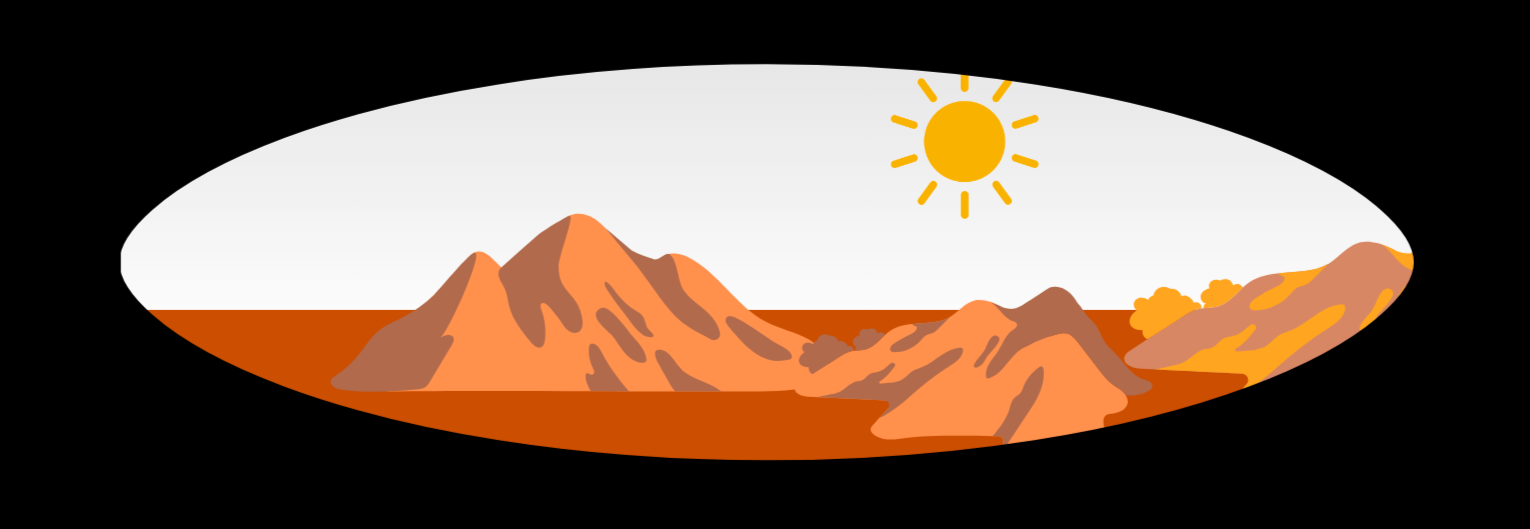
\includegraphics[width=0.5\textwidth]{img/bond_metaphor_desert.png}
%  \caption{Corpus-attested lexicalized metaphors for many languages: a range of views}\label{fig:multi}
\end{frame}


\begin{frame}{Measure the translation overlap with OMW}

  \begin{itemize}
  \item For every English word that has been annotated
    \begin{itemize}
    \item For each pair of English senses
    \item Look up all translations of each sense
      \\ measure the overlap (we use Jaccard similarity)
      \item Store and note if the senses are linked or not
    \end{itemize}
  \item So for example \eng{head} has 3 senses (really many more)
    \begin{enumerate}
    \item head, caput
      \\ ヘッド, \ul{頭}, 頭部 
    \item head, chief, top dog
      \\ 大頭, 主任者, 御頭, 頭領, \ul{頭}
    \item head,  head word
      \\ 主要語
    \end{enumerate}
  \item Overlap
    \begin{itemize}
    \item 1-2: 0.125 %(/ 1.0  8) 0.125
    \item 2-3: 0
    \item 1-3: 0
    \end{itemize}
  \end{itemize}
  

\end{frame}

\begin{frame}[allowframebreaks]{We do this for all the lexicons in OMW-1.4}

 
  \begin{center}
  \begin{tabular}{lrrrr}
    Lang & Unlinked & Metaphor & Metonomy & Non-Zero Instances \\ \hline
sv & 0.70 & 1.71 & 2.10 & 417   \\
he & 0.69 & 1.58 & 2.31 & 472   \\
eu & 0.82 & 1.30 & 1.80 & 5,562  \\
ja & 0.89 & 1.11 & 1.55 & 8,130 \\
ro & 0.83 & 1.30 & 1.71 & 6,429 \\
sq & 0.74 & 1.27 & 2.38 & 822 \\
%en & 0.97 & 1.08 & 1.07 & 33415 \\
da & 0.74 & 1.46 & 2.09 & 332 \\
lt & 0.63 & 1.46 & 2.86 & 692 \\
 \end{tabular}
\end{center}

\begin{itemize}
\item \txx{unlinked} has no link
\item \txx{metaphor} is linked by metaphor
\item \txx{metonymy} is linked by metonymy
\end{itemize}
Normalize by dividing  by the average distance for all senses.

  \begin{center}
  \begin{tabular}{lrrrr}
    Lang & Unlinked & Metaphor & Metonomy & Non-Zero Instances \\ \hline
es & 0.85 & 1.17 & 1.79 & 5,915 \\
 hr & 0.81 & 1.22 & 1.98 & 3,576 \\
    fr & 0.94 & 1.10 & 1.25 & 18,975 \\
nb & 0.73 & 1.49 & 2.12 & 339 \\
bg & 0.73 & 1.54 & 2.11 & 380 \\
gl & 0.70 & 2.13 & 1.55 & 271 \\
cmn & 0.74 & 1.57 & 1.97 & 1,347 \\
it & 0.80 & 1.39 & 1.81 & 4,614 \\
arb & 0.74 & 1.28 & 2.38 & 1,337 \\
pl & 0.75 & 1.43 & 2.07 & 1,326 \\
el & 0.72 & 1.30 & 2.45 & 1,274 \\
iwn & 0.79 & 1.46 & 1.80 & 968 \\
nn & 0.73 & 1.52 & 2.10 & 340 \\
id & 0.87 & 1.21 & 1.58 & 9,803 \\
  \end{tabular}
\end{center}

    \begin{center}
      \begin{tabular}{lrrrr}
    Lang & Unlinked & Metaphor & Metonomy & Non-Zero Instances \\ \hline
is & 0.73 & 1.51 & 2.13 & 388 \\
ca & 0.83 & 1.23 & 1.84 & 6,000 \\
sk & 0.73 & 1.35 & 2.31 & 2,067 \\
fi & 0.82 & 1.35 & 1.76 & 7,971 \\
nl & 0.79 & 1.38 & 1.90 & 2,991 \\
sl & 0.81 & 1.41 & 1.74 & 6,243 \\
th & 0.80 & 1.48 & 1.71 & 2,336 \\
pt & 0.80 & 1.26 & 1.96 & 5,414 \\
        zsm & 0.87 & 1.22 & 1.60 & 10,272 \\
        \midrule
Mean & 0.78 & 1.39 & 1.96 &  3,774\makebox[0mm]{~~~.3} 
  \end{tabular}
    \end{center}
    
  Unlinked  share fewer translations, metaphor shares more and metonomy shares much more.

  \Large Metonomy is more likely to hold cross linguistically!
  
\end{frame}

\begin{frame}{Discussion}

  \begin{itemize}
  \item The wordnets are of vastly different sizes: the number of sense
    pairs that have a translation varies from 271 (Galician) to 18,975 (French). 
  \item   Only Galician has the     score for metaphor (2.13) larger the score for metonymy (1.55), probably due to data sparsity. We would expect it to behave much like
    Portuguese (1.26/1.96).
  \item In order to measure perfectly how well tropes carry
    over between languages, we would need to mark metonymy and metaphor
    systematically for each language, and make sure all synsets for all
    senses have all relevant translations, \ldots 
  \item Without exception, senses linked by tropes are more likely to have an identical translation that those senses which are not linked
  \item With one exception, metonymy is more likely to have  an identical translation then metaphor  
  \end{itemize}

\end{frame}

\begin{frame}{Translations of the senses of \protect\eng{cherry}}
  \begin{center}
 \small 
  \begin{tabular}{llllll}% \toprule
    Sense & Mandarin & Japanese & Finnish & Italian & Portuguese \\ \midrule

    \sense{cherry}{1}   & 樱桃木 & 桜,   \ul{桜材} & kirsikkapuumetsä & ciliegio  & cerejeira \\ 

    \sense{cherry}{2}  & 樱桃树 & 桜, 櫻 & kirsikkapuu & ciliegio  &  cerejeira\\

    \sense{cherry}{3}  & 樱桃  & 桜桃, 桜ん坊 & kirsikka & cerasa , ciliegia  & ginja , cereja \\ 
    
    \sense{cherry}{4} &  \ul{樱桃红} & \ul{桜ん坊色}   &  kirsikanpunainen & ciliegia,  rosso ciliegia & cereja\ %\bottomrule
  \end{tabular}
\end{center}

\begin{itemize}
\item When we look at the translations, we see that the metonymy that is unmarked in English, is marked in other languages
\item Even within English, other synonyms have information
\end{itemize}

\end{frame}



\begin{frame}{Ongoing Research to Find Patterns}
  
\begin{itemize}
\item We can make a searchable database where the edges are decorated by the morphological differences
  \begin{itemize}
  \item So we can see all pairs linked by \dff{en:+ tree} or \dff{da:+træ} 
  \item The nodes link to synsets, so we can look
    up supertypes: we can say this link is of type  \lnk{food:plant}
  \\ or  \lnk{plant is food} in the cognitive linguistic style
  \item In this way we can group the tropes together in families
  \item Similar to \citet{Stoyanova:Mititelu:Leseva:Iordachioaia:2025}
  \end{itemize}
\item Other people have done this top down \cite[e.g start at \lnk{food:plant} and looked for examples]{khishigsuren_bella_brochhagen_marav_giunchiglia_batsuren_2022} 
\item With ChainNet we can go bottom-up and find many more patterns
  \begin{itemize}
  \item We can use multi-lingual features
  \item We need to investigate methods of clustering
  \item We need to find a good way of evaluating
  \end{itemize}
\item We would like to also map to existing Conceptual Metaphors
\end{itemize}

\end{frame}

\begin{frame}{The Patterns can be used Generatively}
  \begin{itemize}
  \item If we see a word that is of type \lnk{food}, then we can expect that
    there may be a kind of plant using the same word
    \begin{itemize}
    \item Useful for analyzing texts that otherwise don't make sense
    \item Can be used to analyse humour and word play \\
    \end{itemize}
  \end{itemize}

  \begin{center}
    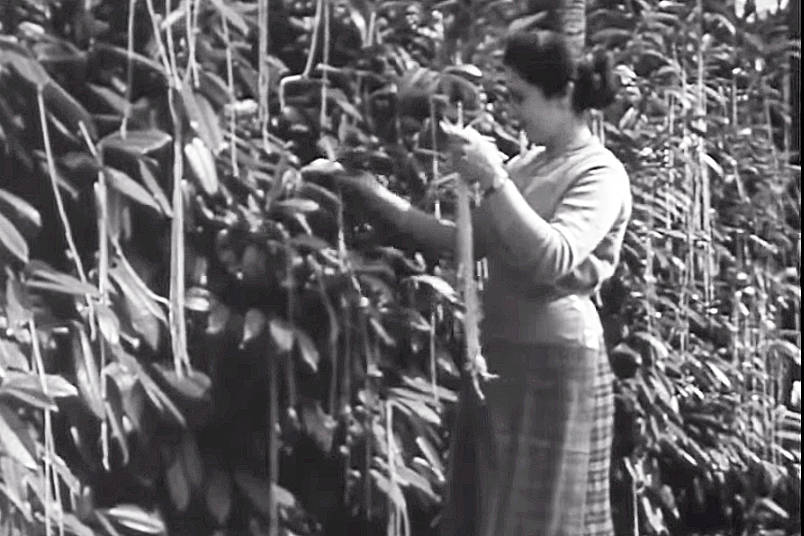
\includegraphics[width=0.5\textwidth]{img/spaghetti-tree.png} \\
    \href{https://en.wikipedia.org/wiki/Spaghetti-tree_hoax}{BBC Spaghetti Tree hoax (1957)}
  \end{center}
\end{frame}



\begin{frame}[p]{Metaphor viewed through the lexicon linked to corpora: a richer view}
  \centering
  
\includegraphics[width=0.9\textwidth]{img/bond_metaphor_plain.png}
%  \caption{Metaphor viewed through the lexicon linked to corpora: a richer view}\label{fig:corpus}
\end{frame}



  

\section{Wordnets}
\begin{frame}
\frametitle{Introduction to Wordnets}

\begin{itemize}
    \item A wordnet is a lexical database that organizes words into sets of synonyms, called synsets.
    \item Each synset represents a unique concept,
      \\ capturing different senses of a word.
    \item Synsets are connected by semantic relations like hypernyms (superordinate) and hyponyms (subordinate).
    \item Wordnets are used in linguistic research, natural language processing (NLP), artificial intelligence, education and (a bit) language maintenance.
\end{itemize}
\end{frame}

\begin{frame}
\frametitle{History of Wordnets}

\begin{itemize}
\item Wordnet was first developed for English at Princeton University \citep{miller1995wordnet}.
  
    \item It was designed it as a model of human lexical memory.
    \item It became a foundational tool for computational linguistics and NLP.
    \item It has influenced the development of lexical resources for many other languages.
    \item Currently the Open English WordNet is maintained by John
      McCrae.  It is extending and revising the Princeton Wordnet.
\end{itemize}
\end{frame}

\begin{frame}{Wordnet Relations}
  \begin{itemize}
  \item Constitutive
    \\  \wn{driver}{n}{1} \rel{hyponym} \wn{operator}{n}{1}
    \\  \wn{driver}{n}{1} \rel{antonym} \wn{nondriver}{n}{1}
    \\   \wn{driver}{n}{3} \rel{synonym} \wn{number one wood}{n}{1}	  
   \\   \wn{golf club}{n}{1} \rel{meronym} \wn{clubhead}{n}{1}	  
  \item Derivational
    \\  \wn{driver}{n}{1} \rel{derived} \wn{drive}{v}{1} 
  \item Descriptive
    \\ \wn{driver}{n}{2} \rel{domain} \wn{computer science}{n}{1}
  \item Implied (from e.g. definitions)
    \\ \wn{driver}{n}{1} ``the \wn{operator}{n}{1} of a \wn{motor
      vehicle}{n}{1}''
    \\ \wn{driver}{n}{2} ``a \wn{program}{n}{3} that
    \wn{determines}{v}{2} how a \wn{computer}{n}{2} will
    \wn{communicate}{n}{1} with a \wn{peripheral device}{n}{1}''
  \end{itemize}
  Over 30 relations are defined, and more are being added \\
  (such as \rel{metaphor}, \rel{metonymy}, \ldots)
\end{frame}


\begin{frame}{The synset for  \eng[tiger]{虎}}
 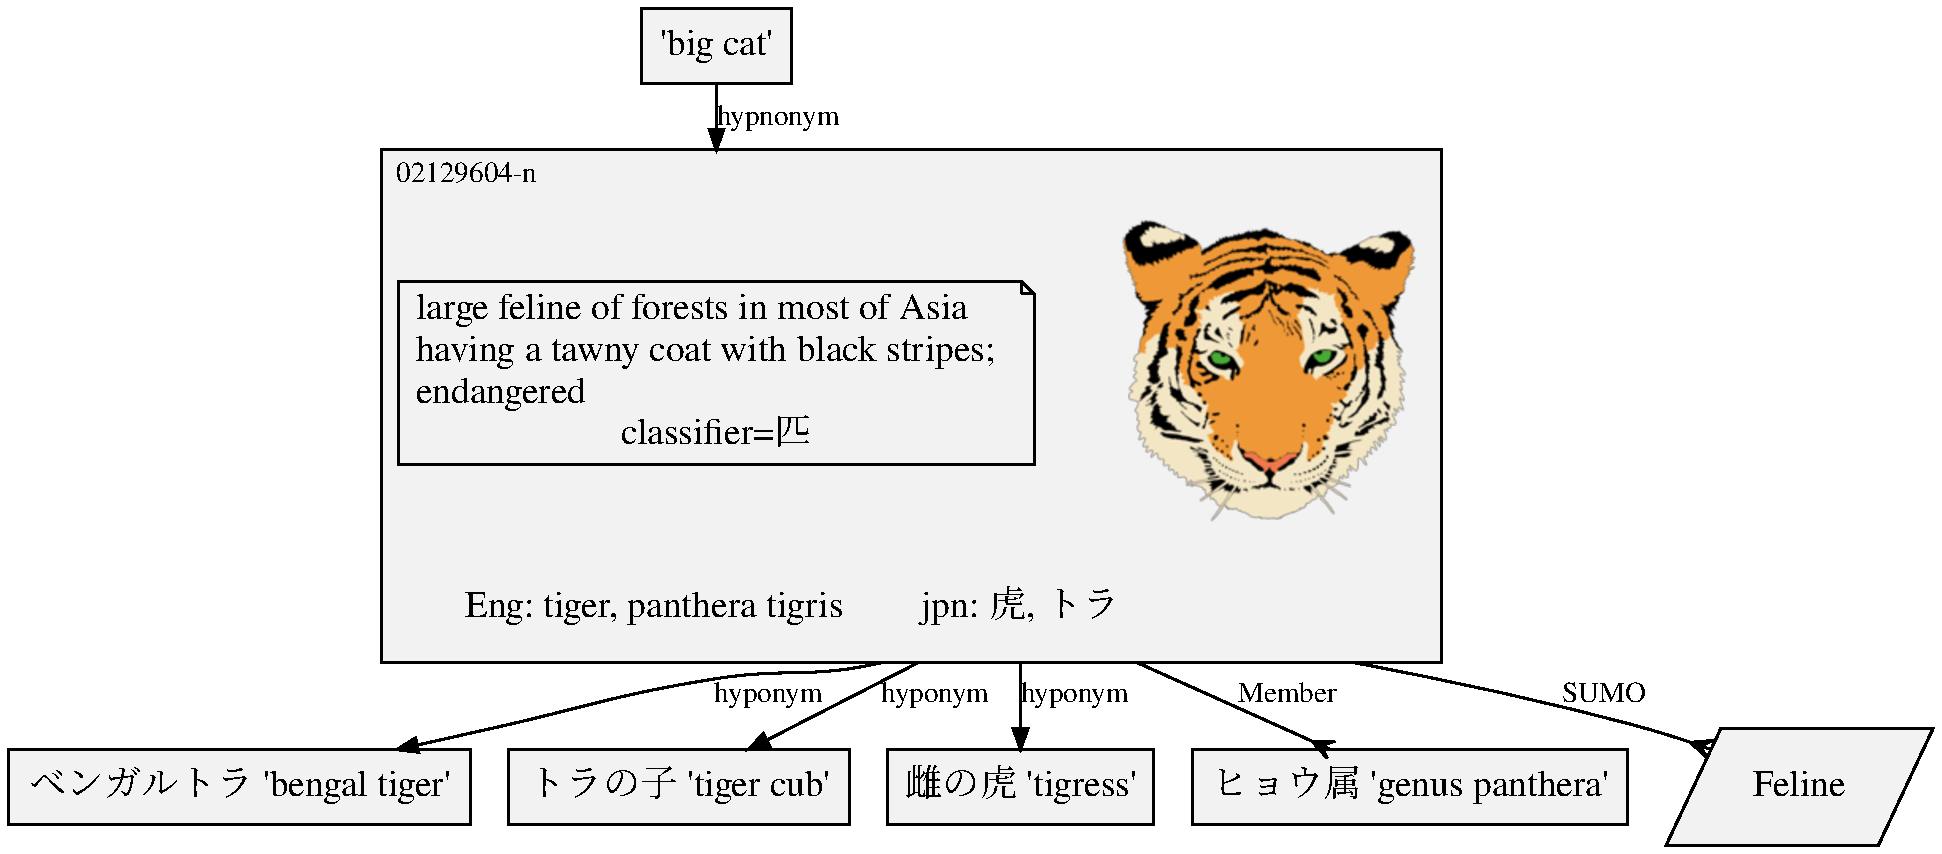
\includegraphics[width=0.9\textwidth]{img/wn-jpn-tiger.pdf}
\end{frame}

\begin{frame}
\frametitle{Wordnet as a Graph}

\begin{itemize}
    \item Synsets can be represented as nodes, and semantic relations as edges.
    \item Hypernymy links form a hierarchical tree, with more general concepts at higher levels.
      \begin{itemize}
      \item Actually a directed acyclic graph, as multiple inheritance is possible
      \end{itemize}
    \item Wordnets also include lateral connections like meronyms and antonyms.
    \item The graph structure allows for efficient computation of semantic similarity.
    \item Graph-based algorithms are used in tasks like word sense disambiguation and knowledge extraction.
\end{itemize}
\end{frame}



\begin{frame}{Usage}
  \begin{itemize}
  \item Wordnets are used for 
    \begin{itemize}
    \item studying word similarity 
    \item describing the meaning of texts
    \item testing WSD algorithms
    \item improving parse ranking
    \item machine translation (not so much these days)
    \item puzzle generation and solving
    \item joke generation
    \item distinguishing senses for word embeddings
    \item language learning
    \end{itemize}
  \item They are still useful in the age of LLMs
    \begin{itemize}
    \item As a check on quality
    \item For explicit reasoning
    \item For languages with insufficient language data
    \item For teaching
    \item For vocabulary-wide testing
    \end{itemize}
  \end{itemize}

\end{frame}

\begin{frame}
\frametitle{Multilingual Wordnets}

\begin{itemize}
    \item    Over 50 hand built wordnets 
    \item Automatically-built Wordnets exist for over 1,200 languages \\ from Swadesh, Wiktionary and more
    \item Cross-lingual mappings help in tasks like machine translation and multilingual semantic analysis.
    \item he Open Multilingual Wordnet (OMW) provide free access to linked open wordnets.
\end{itemize}
\end{frame}

\begin{frame}
\frametitle{Challenges in Building Wordnets}

\begin{itemize}
    \item Developing wordnets requires careful analysis \\ impossible to automate
    \item Word meaning can be culturally specific, \\ requires careful consideration of local concepts.
    \item Data collection for under-resourced languages often involves fieldwork and expert collaboration.
    \item Validation and refinement of synsets is an ongoing process, especially for evolving languages.
    \item Many language resources are not open, so data cannot easily be shared.
\end{itemize}
\end{frame}

% \begin{frame}
% \frametitle{Building Wordnets for Under-resourced Languages}

% \begin{itemize}
%     \item Under-resourced languages may lack dictionaries, corpora, or standardized orthographies.
%     \item Wordnets for these languages require extensive collaboration with native speakers.
%     \item Data collection can involve workshops, interviews, and domain-specific lexicons.
%     \item Wordnet development can support language preservation and revitalization efforts.
%     \item These wordnets help document endangered languages and make them accessible for future research.
% \end{itemize}
% \end{frame}

\begin{frame}
\frametitle{Open Multilingual Wordnet (OMW)}

\begin{itemize}
    \item OMW is a free multilingual lexical database linking wordnets from many languages \citep{Bond:Foster:2013}
    \item OMW includes wordnets for widely spoken languages
    \item It also contains wordnets for under-resourced and endangered languages
    \item Researchers can access and contribute to OMW to support cross-linguistic studies
    \item The platform promotes collaborative development and data sharing across language communities
    \item In particular it has pushed open-licenses for the wordnets
\end{itemize}
\end{frame}

\begin{frame}{Wordnets in the world 2008}
\begin{center}
   \noindent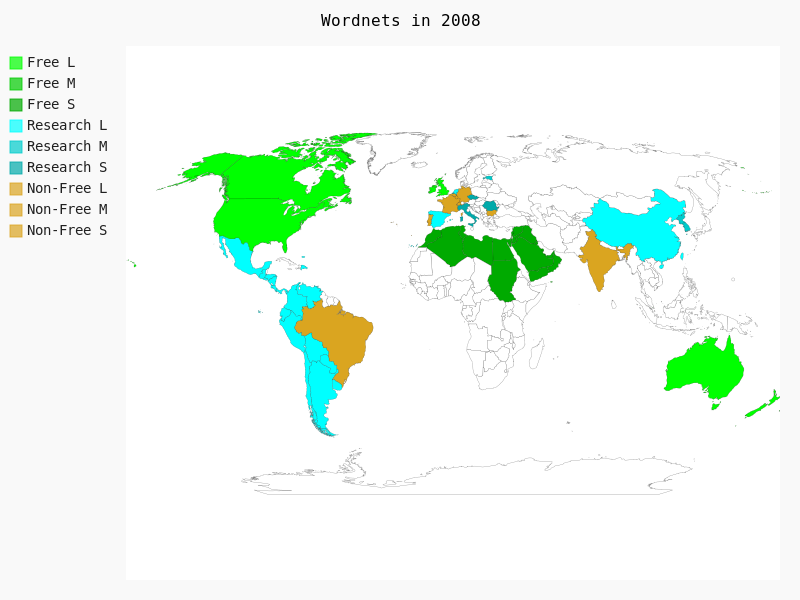
\includegraphics[width=1.0\textwidth]{img/wns-2008}
\end{center}
Green is free; Blue is research only; Brown costs money
\end{frame}

\begin{frame}{Wordnets in the world 2023}
\begin{center}
   \noindent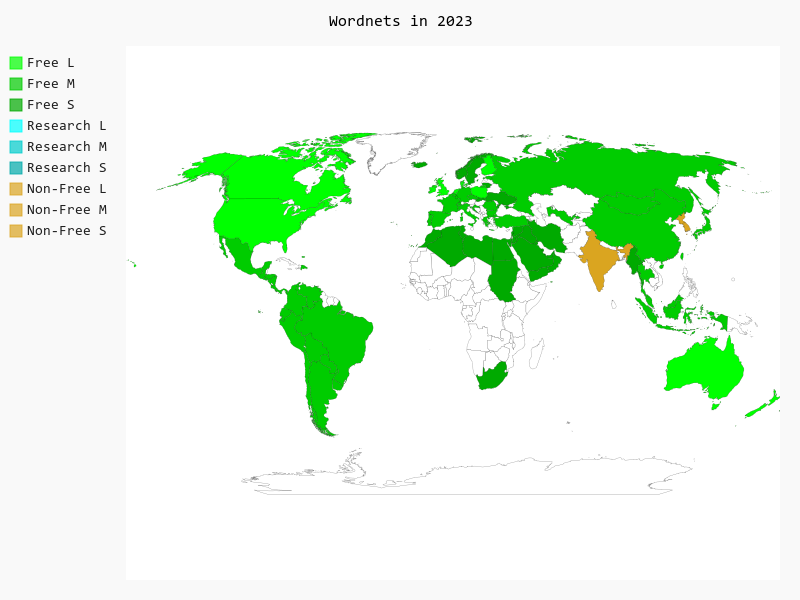
\includegraphics[width=1.0\textwidth]{img/wns-2023}
\end{center}
Green is free; Blue is research only; Brown costs money
\end{frame}

\begin{frame}{The situation is much better!  But not perfect}
  
\begin{itemize}
\item However, it is showing the situation only for the major language for each country
  \begin{itemize}
  \item India has over 450 living languages
  \item Indonesia has over 700 living languages
  \item Australia has over 100 indigenous languages and probably at least that many immigrant languages
  \item Even Czechia recognizes Belarusian, German, Polish, Hungarian, Ukrainian and  Vietnamese as official minority languages
  \end{itemize}
\item We are missing most of the world's languages
  \begin{itemize}
  \item Most wordnets start by exploiting existing resources
    \begin{itemize}
    \item  bootstrap off English
    \end{itemize}
  \item But most of the world's languages do not have lexicons linked
    to English!
  \end{itemize}
\end{itemize}

\end{frame}


% \begin{frame}
% \frametitle{Conclusion of the Introduction}

% \begin{itemize}
%     \item Wordnets are essential resources for understanding the semantic structure of languages.
%     \item They support a wide range of applications in NLP, linguistics, and AI.
%     \item Wordnets are now being developed for many languages, including those with limited resources.
%     \item Multilingual wordnets enable cross-linguistic research and better understanding of language relationships.
%     \item Wordnets contribute to preserving linguistic diversity by documenting and organizing lexical data.
% \end{itemize}
% \end{frame}


\begin{frame}{How are wordnets built?}

  \begin{itemize}
  \item Most new wordnets built be the \txx{expand} method --- the
    structure of Engish is used as a base, and new lemmas are added to the synsets
  \item Some wordnets are built by  the \txx{merge} method --- an existing lexical resources is merged with the English Wordnet
  \item The IndoWordnet \citep{Bhattacharyya:2010} used a clever hybrid
    \begin{itemize}
    \item a new structure was made for Hindi, using existing lexical resources 
    \item other Indic languages used this as a base for expand 
    \item but it is not under an open license, \ldots
    \end{itemize}

  \end{itemize}
  
  
\end{frame}

\section{Low Resource Languages (LRL)}

\begin{frame}
\frametitle{Challenges in Building Wordnets for Low-Resource Languages}

\begin{itemize}
    \item Many languages lack  lexical resources like dictionaries or corpora.
    \item We have to build a foundational lexical database from scratch.
    \item Fieldwork and collaboration with native speakers \\ \ \ \ are essential for data collection.
    \item Cultural and contextual differences make \\  \ \ \ direct translations of concepts difficult.
    \item The lack of standardized orthographies \\  \ \ \ adds complexity to digitization and documentation.
\end{itemize}
\end{frame}

% \begin{frame}
% \frametitle{Data Collection Challenges}

% \begin{itemize}
%     \item Workshops, interviews, and manual documentation are often necessary for word collection.
%     \item Language consultants may be required for translating and interpreting lexical data.
%     \item Typically language experts and computer experts are not the same people.
%     \item Word meanings may vary by dialect or region, making consistent data collection difficult.
%     \item Language communities with no history of standardisation may disagree as to what should be considered correct
%     \item Time and cost constraints limit how much data can be collected.
%       \\ also true for well-resourced languages!
% \end{itemize}
% \end{frame}

% \begin{frame}
% \frametitle{Semantic Structure Challenges}

% \begin{itemize}
%     \item Identifying and organizing synsets in under-resourced languages can be difficult.
%     \item Concepts may not map directly onto concepts in other languages, such as English.
%     \item Cultural concepts and practices often require unique synsets that do not exist in larger languages.
%     \item Expert knowledge of the language's lexical semantics is essential for accurate synset creation.
% \end{itemize}
% \end{frame}

% \begin{frame}
% \frametitle{Technological Challenges}

% \begin{itemize}
%     \item Tools and resources for building wordnets, such as NLP software, are not readily available for low-resource languages.
%     \item Manual annotation and digitization of handwritten data are time-consuming and error-prone.
%     \item Often it is not just that you don't have, for example, a  part-of-speech tagger, but that no-one had yet identified what parts of speech are appropriate
%     \item Collaboration between linguists and native speakers can be logistically challenging without reliable power, internet or software tools.
% \end{itemize}
% \end{frame}

% \begin{frame}
% \frametitle{Sociolinguistic and Cultural Challenges}

% \begin{itemize}
%     \item Some communities may resist linguistic documentation efforts due to concerns about language preservation.
%     \item Native speakers may prioritize language revitalization over computational resources like wordnets.
%     \item The process of documenting a language for a wordnet can introduce external cultural biases.
%     \item[★] Collaboration with local communities is essential to ensure cultural respect and accuracy.
%     \item[★] Ethical considerations are crucial when engaging with endangered language communities.
% \end{itemize}
% \end{frame}

\begin{frame}
\frametitle{Challenges in Data Validation and Accuracy}

\begin{itemize}
    \item Data collected from native speakers will contain inconsistencies or errors.
    \item Language experts are often needed to validate synsets and relations.
    \item Regular updates and revisions are necessary as languages evolve or more data is collected.
    \item Data verification is particularly challenging for languages with no formal linguistic documentation, and few or no collections of text.
\end{itemize}
\end{frame}

\begin{frame}
\frametitle{Community Involvement}

\begin{itemize}
    \item Involving the language community is key to successful wordnet development.
    \item Native speakers contribute cultural and contextual insights critical to building accurate wordnets.
    \item Community workshops help ensure that the wordnet reflects the language as spoken by its speakers.
    \item Community members often play a key role in digitizing and validating the wordnet.
    \item Without community involvement, the wordnet may not reflect the real linguistic and cultural landscape.
\end{itemize}
\end{frame}

\begin{frame}{Wordnet is not designed to cover everything}

  \begin{itemize}
  \item The original Princeton wordnet only covered content words: nouns, verbs, adjectives and adverbs in English
    \begin{itemize}
    \item There was no need to cover every word class --- plenty of other dictionaries do that
    \end{itemize}
  \item But if a language has no dictionary, so the wordnet is going to be the \txx{only} lexicon --- then it needs to cover everything the community needs
      \begin{itemize}
      \item Other parts of speech
      \item Usage notes
      \item Audio
      \item Spelling variation
      \end{itemize}
    \item And the data should be as accessible as possible
      \begin{itemize}
      \item to the community
      \item to the field linguists
      \item to other researchers
      \end{itemize}
  \end{itemize}
  
\end{frame}

%\begin{frame}
  
%  \frametitle{Challenges in Maintaining Wordnets}

% \begin{itemize}
%     \item Maintenance requires continuous updates as the language changes or new words are added.
%     \item Low-resource languages may not have sufficient funding or institutional support for long-term projects.
%     \item Finding skilled annotators or linguists for updates can be difficult in smaller communities.
%     \item Technical infrastructure (e.g., servers, hosting) must be sustained over time to keep the wordnet accessible.
%     \item Support for open-source projects like wordnets may diminish without strong community or academic backing.
% \end{itemize}
% \end{frame}

\begin{frame}
\frametitle{Balancing Preservation and Innovation}

\begin{itemize}
    \item Wordnets can support language preservation efforts by documenting lexical data.
    \item At the same time, they promote technological innovation, enabling computational uses of the language.
    \item There is often tension between focusing on language preservation versus creating resources for NLP applications.
    \item Balancing traditional language documentation with new technological tools is a key challenge.
    \item Wordnets offer a way to bridge the gap between preserving linguistic heritage and advancing technology.
\end{itemize}
\end{frame}

%\begin{frame}
% \frametitle{Conclusion of the Challenges}

% \begin{itemize}
%     \item Building wordnets for languages with limited resources involves complex challenges, from data collection to validation.
%     \item Close collaboration with native speakers and language communities is critical for success.
%     \item Despite these challenges, wordnets play a vital role in documenting, preserving, and revitalizing low-resource languages.
%     \item Addressing both linguistic and technical obstacles ensures that these languages remain accessible for future generations.
%     \item Wordnets contribute to the global linguistic diversity and cultural preservation efforts.
% \end{itemize}
% \end{frame}


\section{Case Studies}

\subsection{Abui}

\begin{frame}
\frametitle{Case Study 1: The Abui Wordnet}

\begin{itemize}
    \item Abui (ISO 639-3: abz, abui1241) is a Timor-AlorPantar (TAP) language \citep{Kratochvil:2007}
    \item Spoken by about 40 thousand speakers in Central Alor
    \item  We worked with the village of Takalelang on the northern coast.
    \item The Abui wordnet was developed as part of a fieldwork project documenting the language.
    % \item Originally the data was stored in SIL toolbox, an NLP tool for field linguists
    % \item Then the collection was expanded using Rapid Word Collection (RWC) workshops with local speakers.
    % \item Words were collected across domains like plants, animals, emotions, and kinship.
    \item Collected data is in the process of being (manually) digitized and structured into a wordnet format.
\end{itemize}
\end{frame}

\begin{frame}{Alor}
\begin{center}
   \noindent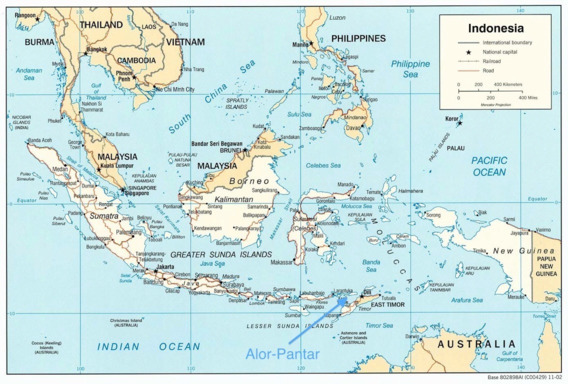
\includegraphics[width=1.0\textwidth]{img/alor-s.png}
\end{center}
\end{frame}

\begin{frame}
\frametitle{Toolbox to wordnet (Version 1)}
 \begin{tabular}{cc}
  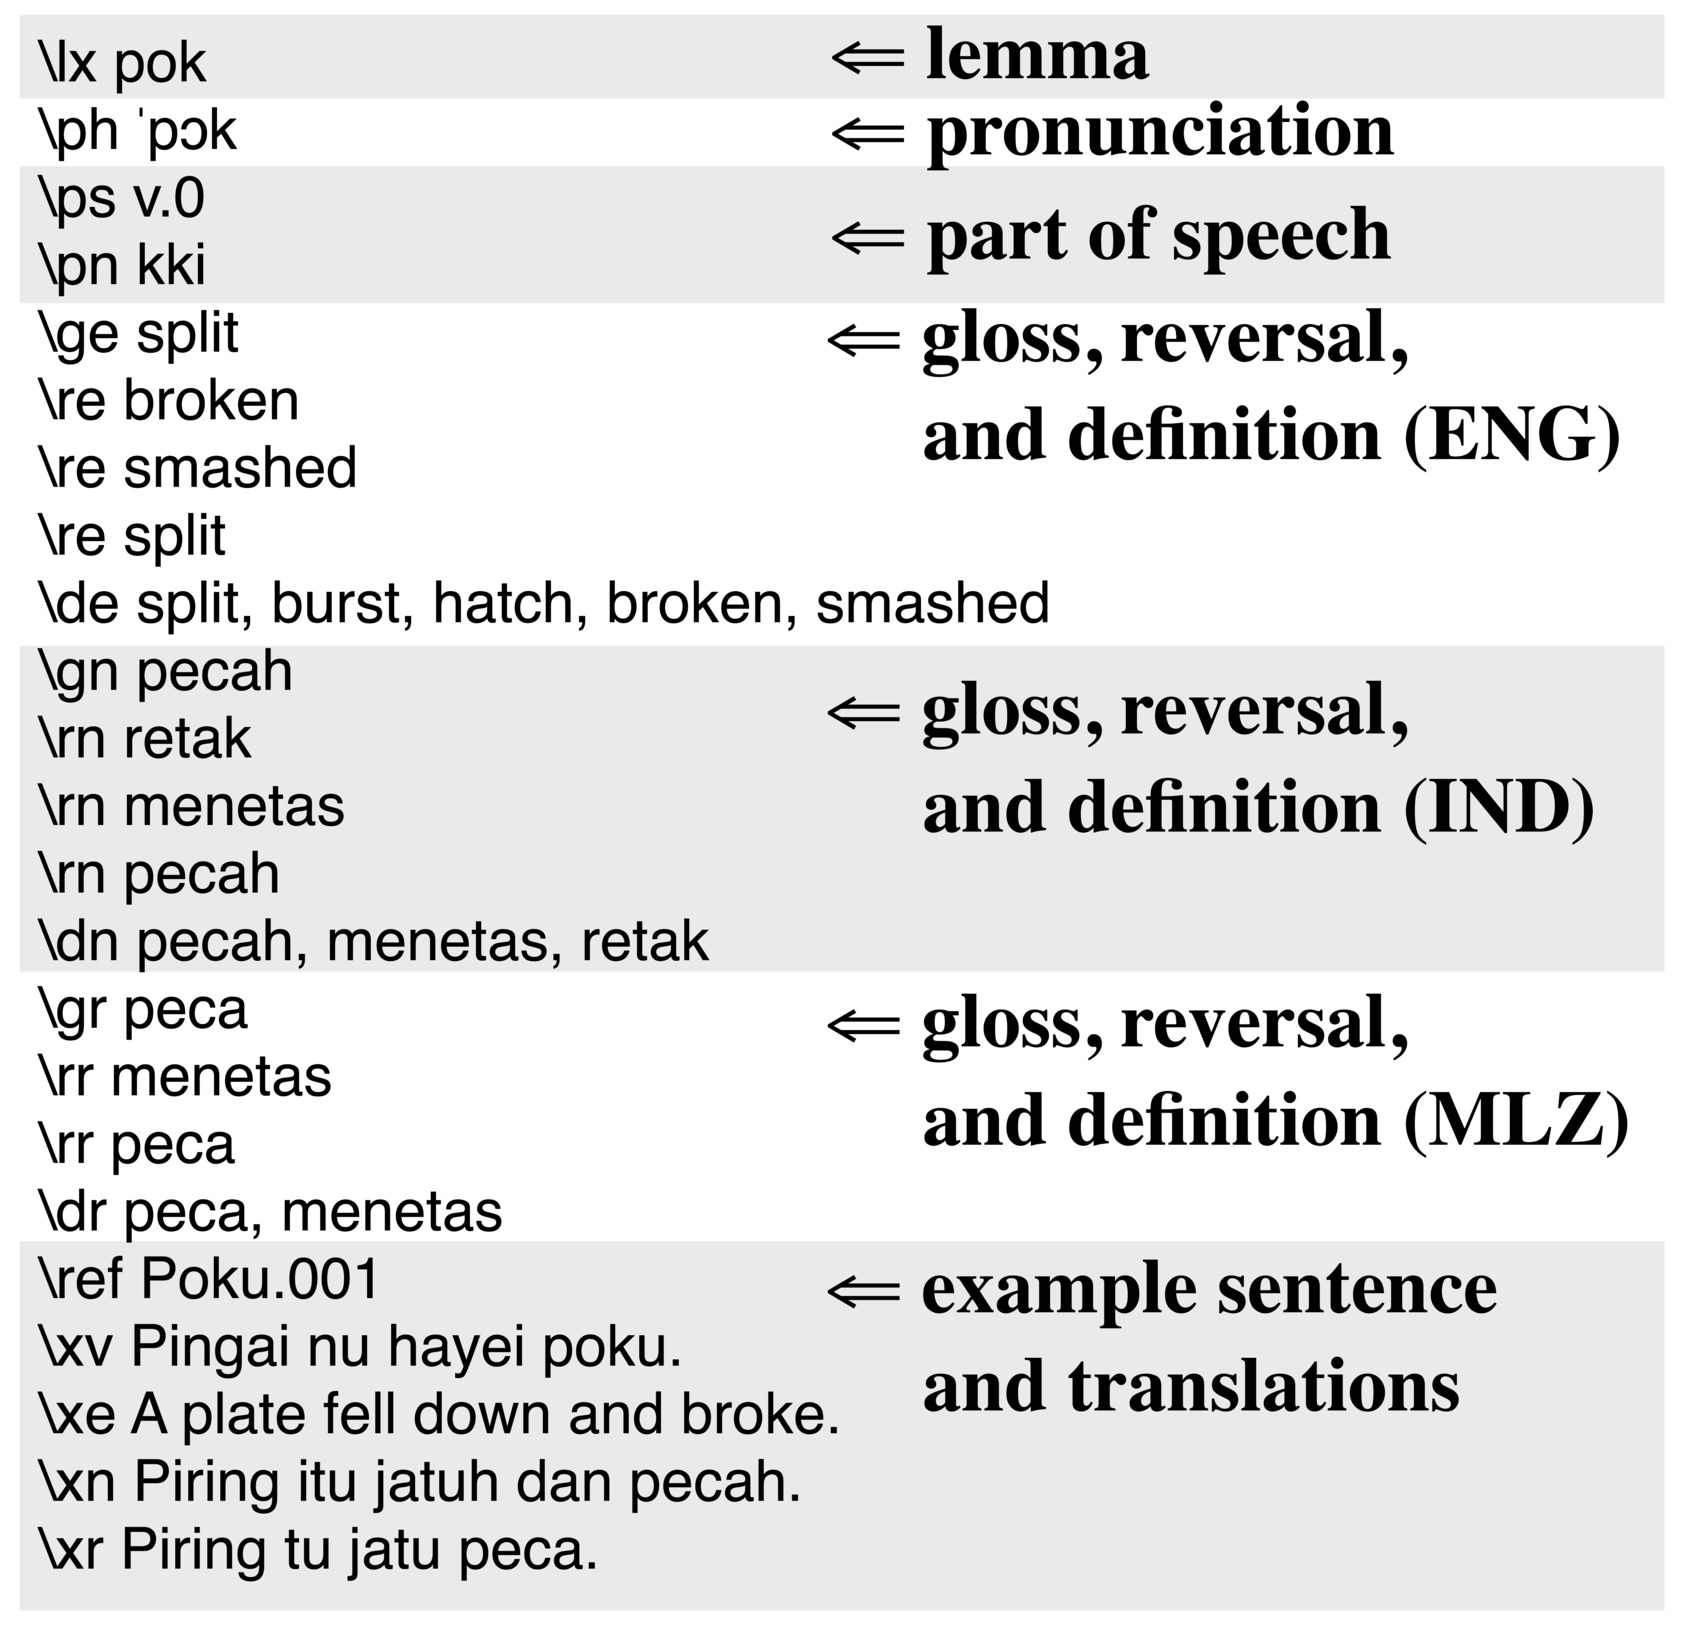
\includegraphics[width=0.4\textwidth]{img/ToolboxDictFormat-s.png}
   &
 \begin{minipage}{0.5\linewidth}
   \begin{itemize}
   \item Uses the glosses to link to English, Malay and Indonesian wordnets
   \item Intersection in 3 language has an accuracy of 0.99, 2 languages around 0.5 and 1 language 0.35
     \begin{itemize}
     \item Even though Malay and Indonesian are very similar!
     \end{itemize}
   \item Data made available at \url{https://github.com/fanacek/abuiwn}
   \item This wordnet was built using other wordnets
   \end{itemize}
   \hfill \citep{kratochvil-morgado-da-costa-2022-abui}
 \end{minipage}
 \end{tabular}
 \end{frame}


\begin{frame}{Rapid Words Construction (Version 2)}
  
\begin{itemize}
    \item But we wanted more words!
    \item Three RWC workshops were conducted with over 80 participants across multiple days.
    \item Workshops focused on gathering words within specific semantic domains.
    \item Participants included native speakers from different parts of the community, ensuring dialectal coverage.
    \item Words were first handwritten, then digitized and annotated for semantic relations.
    \item SIL domains were mapped to wordnet concepts, again using translation overlap \citep{Zulhelmy:Bond:Kratochvil:2014,Costa:Kratochvíl:Saad:Delpada:Lanma:Bond:Wolfová:2023}
      \begin{itemize}
      \item because the granularity is very different they do not often match one-to-one
      \item so there is more manual work to be done
      \end{itemize}
    % \item Collaboration with linguists ensured accurate synset creation and semantic alignment.
\end{itemize}
\end{frame}

\begin{frame}{It was a blast}
  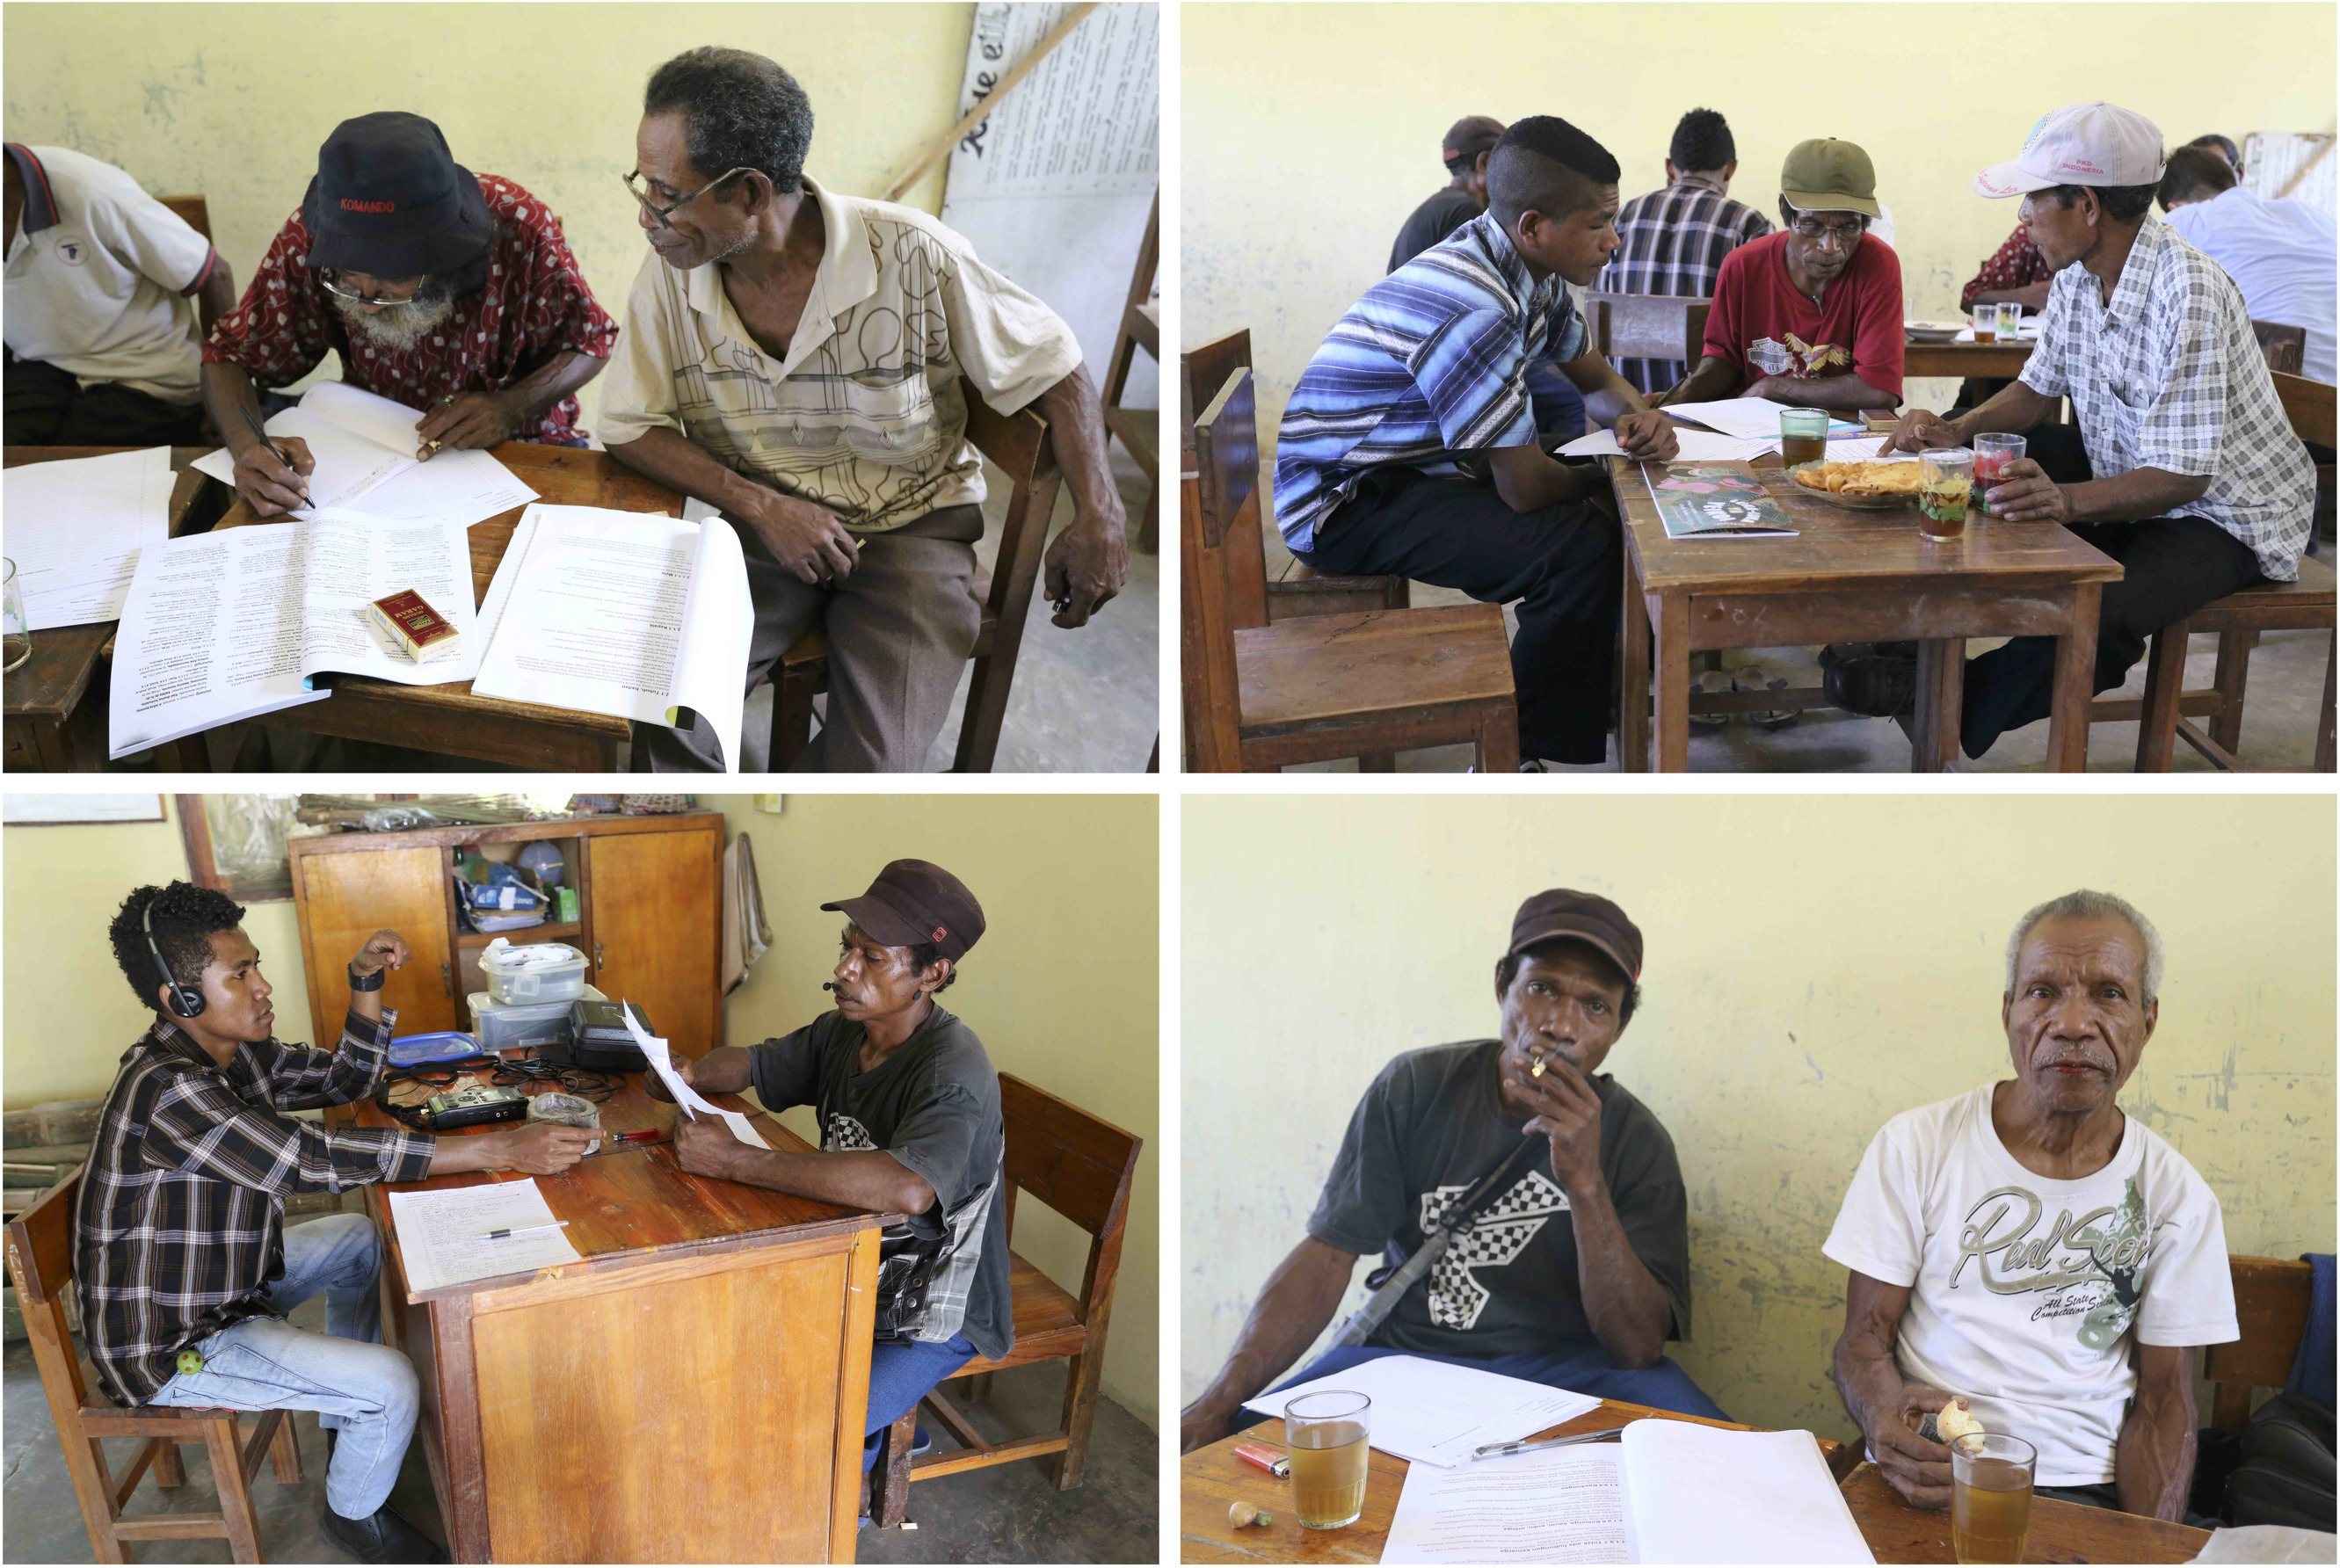
\includegraphics[width=1.0\textwidth]{img/WorkshopSmall-s.jpg}
\end{frame}

\begin{frame}{SIL semantic domain for water (1.3)}
  \begin{tabular}{cc}
    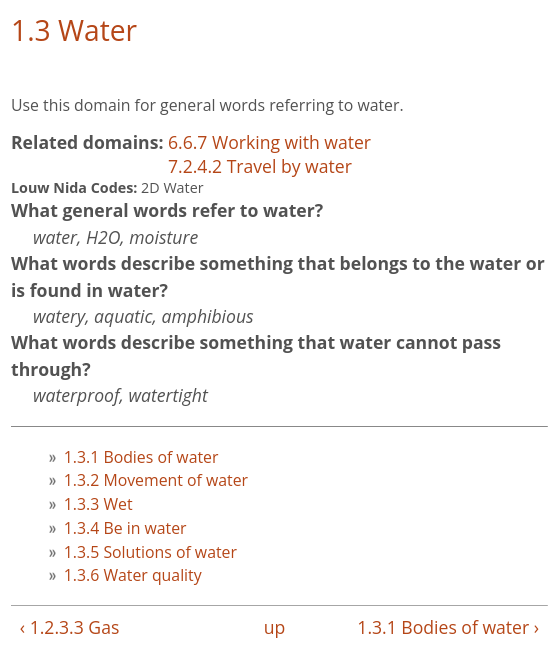
\includegraphics[width=0.4\textwidth]{img/sil-semdom-water.png}
    &
    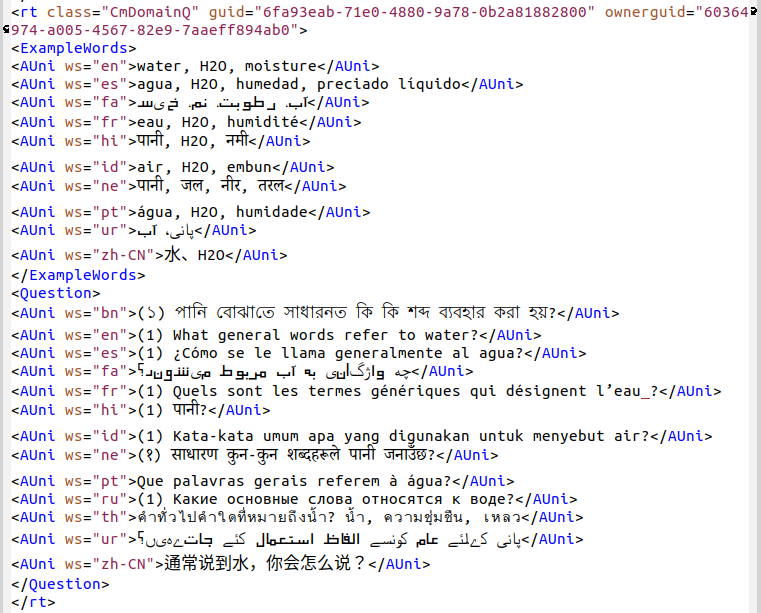
\includegraphics[width=0.6\textwidth]{img/fieldwords-water.png}
      
  \end{tabular}
\end{frame}

\begin{frame}


  \frametitle{Challenges in Building the Abui Wordnet}

\begin{itemize}
\item Data entry was the biggest bottleneck
  \begin{itemize}
  \item Only a native speaker can really digitize the data
  \item There are only a handful who could
  \item They often have other things to do
  \end{itemize}
\item Computational linguist time is also a  bottleneck
  \begin{itemize}
  \item Resource creation is rarely well-funded
  \item It takes second place to other tasks
  \end{itemize}
\item Orthographic variation is also a problem
  \begin{itemize}
  \item The orthography is being refined as we record more data
  \item It is hard to update older data
  \end{itemize}
\end{itemize}
\end{frame}

\begin{frame}
\frametitle{Outcomes of the Abui Wordnet Project}

\begin{itemize}
    \item The Abui wordnet documented over 1,400 synsets and 3,600 senses
    \item A new version with 2,500 synsets is on its way
    \item It serves as a lexical resource for both linguistic research and the local community.
    \item The project supported ongoing language documentation and preservation efforts.
    \item Native speakers have been deeply involved in the project and are training in linguistics
    \item The Abui wordnet was incorporated into the Open Multilingual Wordnet (OMW) project --- you can even find it in hugging face!
 \item We are currently working on annotating a text: \textit{Bukuuting bikaat-bikaat} ``The Speckled Band', which we translated from Indonesian 
 \\ for this we need a lemmatizer, \ldots
    \end{itemize}
\end{frame}

%\begin{frame}
% \frametitle{Significance of the Abui Wordnet}

% \begin{itemize}
%     \item The wordnet highlights the role of collaborative fieldwork in low-resource language documentation.
%     \item It provides a linguistic resource for Abui speakers, researchers, and educators.
%     \item The project helps preserve Abui by recording its lexical structure and key cultural concepts.
%     \item It represents a model for other Papuan and low-resource languages in similar contexts.
%     \item The Abui wordnet demonstrates how modern tools can assist in documenting oral traditions.
%     \item We are currently working on annotating a text: \textit{Bukuuting bikaat-bikaat} ``The Speckled Band', which we translated from Indonesian
% \\ for this we need a lemmatizer, \ldots
% \end{itemize}
% \end{frame}


\subsection{Cantonese}

\begin{frame}
\frametitle{Case Study 2: The Cantonese Wordnet}

\begin{itemize}
    \item Cantonese is spoken by millions, but its written tradition is limited compared to Mandarin.
    \item The Cantonese wordnet project aims to provide a lexical resource for this major Chinese variety.
    \item The Cantonese wordnet includes everyday Cantonese vocabulary, colloquialisms, and slang.
    \item It currently has senses, examples, a small sense-tagged corpus \citep{sio-costa-2019-building,sio:morgadodacosta:2022a}
    \item It also has parts-of-speech not in the original wordnet: classifiers and aspect markers
\end{itemize}
\end{frame}
\begin{frame}{Where is Cantonese (and other Chineses) spoken?}
  \includegraphics[height=0.8\textheight]{img/cantonese-other-chinese-map.png}

  From \citet{Zhenxing:2012}.
\end{frame}


\begin{frame}
\frametitle{Challenges in Building the Cantonese Wordnet}

\begin{itemize}
    \item Cantonese has a strong oral tradition but less standardized written forms.
    \item Because of this there is quite a bit of variation
    \item As Cantonese is a spoken variety, and there is some
      variation in pronunciation, we decided to add audio to the wordnet
      \begin{itemize}
      \item This takes advantage of the extensions to the wordnet format from 2020
      \item As far as we know we are the first people to add sound
      \item We recorded some data ourselves
      \item We harvested some data from Wikicommons
        \begin{itemize}
        \item Many entries were Mandarin with Cantonese pronunciation, not Cantonese
        \item It is difficult to distinguish them
        \item But essential to do so
        \end{itemize}
      \end{itemize}
    \item It was sometimes hard to distinguish words from phrases
      \begin{itemize}
      \item Written Chinese does not show word boundaries
      \item Linguists disagree on what should be a word
      \end{itemize}

\end{itemize}
\end{frame}


\begin{frame}{The OMW interface showing audio}
    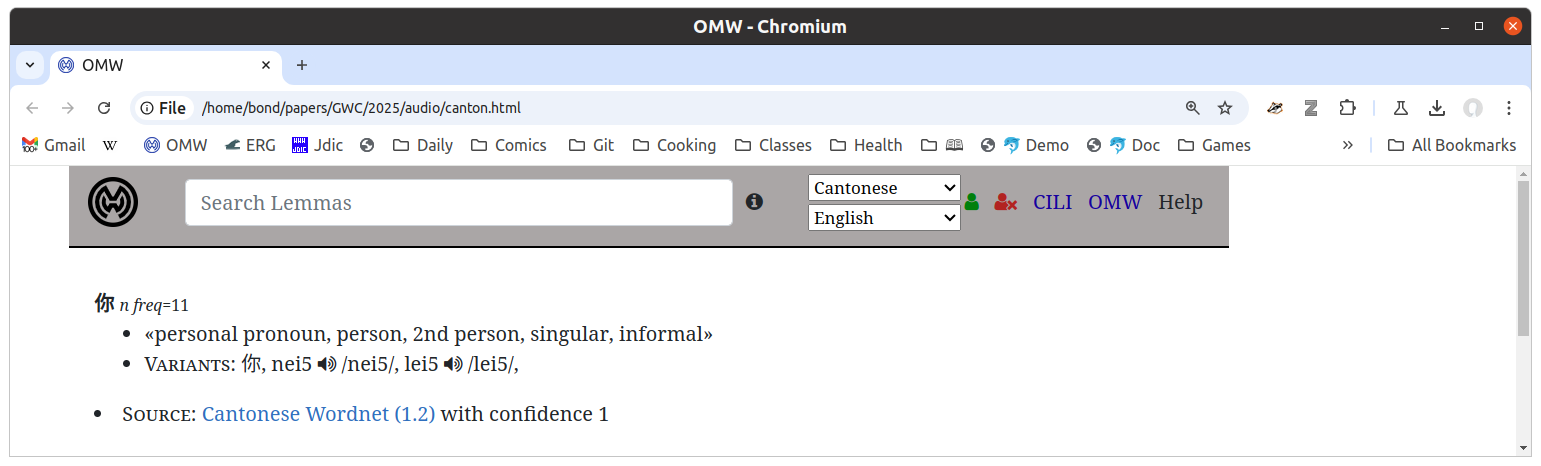
\includegraphics[width=1.0\textwidth]{img/nei5.png}

    \begin{itemize}
    \item This shows a word with two pronunciations
      \begin{itemize}
      \item nei5 is the standard pronunciation
      \item lei5 is the `lazy' pronunciation \citep{Chen:2018}
      \end{itemize}
    \end{itemize}
    
\end{frame}


\begin{frame}
\frametitle{Outcomes of the Cantonese Wordnet Project}

\begin{itemize}
\item The Cantonese wordnet is a carefully curated resource 
  \begin{itemize}
  \item 6,200 concepts
  \item 17,350 senses
  \item 2,138 audio examples, covering 2,859 senses
    % (+ 5250 964) 6214 (+ 16300 1050) 17350
  \end{itemize}
    \item The project aids in preserving Cantonese as a separate linguistic entity from Mandarin.
    \item The wordnet has been used as data to distinguish Mandarin from Cantonese
    \item It serves as a basis for future research on Cantonese language technology development
\end{itemize}
\end{frame}

%\begin{frame}
% \frametitle{Significance of the Cantonese Wordnet}

% \begin{itemize}
%     \item The Cantonese wordnet serves as a reference for the vocabulary of the language.
%     \item It supports the development of linguistic resources for non-Mandarin Chinese varieties.
%     \item The wordnet helps capture the cultural and linguistic identity of Cantonese speakers.
%     \item It contributes to the broader effort of documenting and preserving regional Chinese languages.
%     \item The project highlights the importance of creating linguistic resources for spoken varieties.
% \end{itemize}
% \end{frame}

\section{Advantages and disadvantages of using wordnets for LRL}

\begin{frame}
\frametitle{Advantages of Wordnets for Low-Resource Languages}

\begin{itemize}
    \item Wordnets help document and preserve linguistic data for endangered or under-documented languages.
    \item They enable cross-linguistic comparison by aligning synsets with wordnets of other languages.
    \item Wordnets provide a structured, searchable resource that benefits researchers and language communities.
    \item They can be used to support language revitalization efforts and to create educational materials.
      \begin{itemize}
      \item Having an online presence can boost the social-status of a language
      \end{itemize}
    \item Wordnets help build other wordnets
      \begin{itemize}
      \item More languages allows better bootstrapping
      \item Phenomena covered in one language make it easier for the next
      \item The more data there is, the better the descriptions become
      \end{itemize}
\end{itemize}
\end{frame}

\begin{frame}
\frametitle{Cultural and Linguistic Preservation}

\begin{itemize}
\item Wordnets should record and organize culturally significant concepts that may not exist in other languages.
  \begin{itemize}
  \item \emp{This has not been done as much as it should}
  \item Adding and describing new concepts is the next great challenge!
  \end{itemize}
    \item They create a permanent record of a language's lexicon, supporting long-term preservation.
    \item Wordnets reflect the unique cultural and cognitive world of speakers, documenting traditional knowledge.
    \item In endangered languages, wordnets can capture the lexical heritage before it disappears.
    \item They facilitate the transmission of traditional vocabulary to younger generations.
\end{itemize}
\end{frame}

\section{Metaphors}






\begin{frame}{Metaphor in Large Language Models}
  \begin{itemize}
  \item Because these tropes are so established, LLMs capture the
    patterns well, and can generalise to novel examples, at least for languages with a lot of online data
  \item E.g. For Spanish, \citet{puraivan2024metaphor} found ChatGPT
    could differentiate literal from metaphorical senses with an
    accuracy of 85-88\% (on a small dataset)
    \begin{itemize}
    \item This is high enough to cause \txx{automation blindness}
    \item It is very hard for a human to spot mistakes
    \end{itemize}
  \item Recent research shows that this accuracy goes down for
    languages with less data and for less common senses
  \item There are also interesting questions of how much metaphor
    interpretation in multilingual models is effected by other languages
    \\ The DanNet group have found metaphors in Danish not found in English are less likely to be recognized
  \item So it is important to
    keep working on producing reliable
    manually annotated data
  \end{itemize}%     

  
 \end{frame}


\begin{frame}{A metaphor of our research!}

  \begin{center}
  
\includegraphics[width=0.75\textwidth]{img/bond_metaphor_diagram_1.png}

  The state-of-the-art: scattered fragments


\includegraphics[width=0.75\textwidth]{img/bond_metaphor_plain.png}

A systematic collection: a richer view

\end{center}
\end{frame}

\begin{frame}{Summary}
  
\begin{itemize}
\item The combination of detailed annotation of meaning and
  cross-lingual links allow us to explore differences in meaning
  representation
  \begin{itemize}
  \item  Metonymy is based on association and contiguity
    \\ \txx{more universal}
  \item  Metaphor often requires analogical reasoning and cultural framing
    \\ \txx{more culture and language specific}
  \end{itemize}
\item We don't know if the tropes are independently discovered, come from a common ancestor, or are borrowed (the same problem as with cognates in etymology)

\item LLMs may capture these regularities, but are hard to explore with
\item Open shared lexicons allow us to look across languages
\end{itemize}

\end{frame}



\section{Thanks}

\begin{frame}{Thanks and disclaimer}

  \begin{itemize}
  \item Thanks to RegICON and Shikhar Kr Sarama for inviting me to present this work
  \item Parts of this talk were presented at the Teanga Project and the Sprogteknologisk Konference 2024
  \item Thanks to all the many people who have worked on these
    resources, especially  Rowan Hall Maudslay, František Kratochvíl, Luís Morgado da Costa and Joanna Ut-Seong Sio.
  \item I have talked about projects my lab has been involved in, as I know them best, but there are many other wordnets for LRL
    \begin{itemize}
    \item Amharic, Kurdish, Mansi, Moroccan Arabic, Sardinian, ASL, Uzbek, Welsh, Bodo, \ldots
    \end{itemize}
  \item There are also wordnets for ancient languages \begin{itemize}
    \item Ancient Greek, Coptic, Latin, Qin Chinese, Sanskrit\ldots
    \end{itemize}
  \item If you are interested in wordnets or metaphor, come and talk to me!
  \end{itemize}


  
\end{frame}


\begin{frame}[allowframebreaks]
        \frametitle{References}
        \bibliographystyle{aclnat}
        \bibliography{abb,mtg,ling,nlp}
\end{frame}



\end{document}

%%% Local Variables: 
%%% coding: utf-8
%%% mode: latex
%%% TeX-PDF-mode: t
%%% TeX-engine: xetex
%%% End: 
